\documentclass{article}
\usepackage{graphicx} % Required for inserting images
\usepackage{multicol}
\usepackage[shortlabels]{enumitem}
\usepackage{listings}
\usepackage{xcolor}
\usepackage{inconsolata}

\lstset{
    basicstyle=\ttfamily\color{red},
    language=C++,
}

\title{
Algoritmos e Estrutura de Dados PCO001

Resolução de: \textbf{Exercícios - Pilha}
}
\author{Carlos Augusto Ribeiro}
\date{2024-01}

\begin{document}

\maketitle

\par
\noindent
\textbf{Tarefa 1} - Considerando a Figura 1, apresente a sequência de operações empilha e desempilha que devem ser aplicadas sobre as pilhas X, Y e Z para que, partindo do estado inicial, possamos chegar ao estado final.

\begin{figure}[h!]
    \clearpage
    \centering
    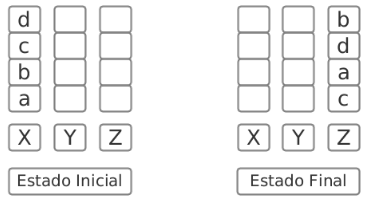
\includegraphics[width=0.5\linewidth]{pilha/1.PNG}
    \caption{Estado inicial e final das pilhas X, Y e Z.
}
\end{figure}

\par
\noindent
\textbf{Solução}
\begin{multicols}{2}
\color{red}
\begin{enumerate}
    \item desempilha X
    \item empilha Y
    \item desempilha X
    \item empilha Y
    \item desempilha X
    \item empilha Z
    \item desempilha Y
    \item empilha Z
    \item desempilha X
    \item empilha Z
    \item desempilha Y
    \item empilha Z
\end{enumerate}
\end{multicols}

\bigskip

\par
\noindent
\textbf{Tarefa 2} - Considere as seguintes funções:
\begin{itemize}
    \item \textbf{Push(P, a)}: Aumenta o tamanho da pilha \textbf{P}, acrescentando o elemento a no seu topo (empilha);
    \item \textbf{Pop(P)}: Remove e retorna o elemento que está no topo da pilha \textbf{P} (desempilha);
    \item \textbf{Top(P)}: Retorna o elemento do topo da pilha \textbf{P}, sem desempilhar.
\end{itemize}

\par
\noindent
Observe a seguir como estas operações interagem para alterar o estado de uma pilha \textbf{P}, inicialmente vazia (\textbf{P[]}), cuja extremidade esquerda foi escolhida como topo. Por exemplo, imagine a pilha \textbf{P} com os elementos \textbf{[r,g]}. Ao executar o comando \textbf{Push(P,b)}, a pilha P ficaria \textbf{[b,r,g]}.
\begin{enumerate}[(a)]
    \item Push(P,a); \( \rightarrow \) \textcolor{red}{[a]}
    \item Push(P,Pop(P)); \( \rightarrow \) \textcolor{red}{[a]}
    \item Push(P,b); \( \rightarrow \) \textcolor{red}{[b,a]}
    \item Pop(P); \( \rightarrow \) \textcolor{red}{b} \( \rightarrow \) \textcolor{red}{[a]}
    \item Push(P,c); \( \rightarrow \) \textcolor{red}{[c,a]}
    \item Push(P,e); \( \rightarrow \) \textcolor{red}{[e,c,a]}
    \item Push(P,Top(P)); \( \rightarrow \) \textcolor{red}{[e,e,c,a]}
    \item Pop(P); \( \rightarrow \) \textcolor{red}{e} \( \rightarrow \) \textcolor{red}{[e,e,c,a]}
\end{enumerate}

\bigskip

\par
\noindent
\textbf{Tarefa 3} - Considere uma pilha \textbf{P} de valores inteiros. Implemente uma função que apresenta o número de elementos contidos em P.\\
\textbf{Protótipo}: int TamanhoPilha (Pilha).

\bigskip
\par
\noindent
\textbf{Solução}
\begin{lstlisting}
int TamanhoPilha(Pilha &pilha) {
    int tamanho = 0;
    char elemento;
    Pilha aux; IniciaPilha(aux);
    while (Desempilha(pilha, elemento)) {
        tamanho++;
        Empilha(aux, elemento);
    }
    while (Desempilha(aux, elemento)) {
        Empilha(pilha, elemento);
    }
    return tamanho;
}
\end{lstlisting}

\bigskip

\par
\noindent
\textbf{Tarefa 4} - Considere uma pilha \textbf{P} de valores inteiros. Implemente uma função que apresenta a média dos valores contidos em \textbf{P} (Figura 2).\\
\textbf{Protótipo}: float MediaPilha (Pilha).
\bigskip
\par
\noindent
\textbf{Solução}
\begin{lstlisting}
float MediaPilha(Pilha &pilha) {
    int tamanho = 0;
    float sum = 0;
    int elemento;
    Pilha aux; IniciaPilha(aux);
    while (Desempilha(pilha, elemento)) {
        tamanho++;
        sum+=elemento;
        Empilha(aux, elemento);
    }
    while (Desempilha(aux, elemento)) {
        Empilha(pilha, elemento);
    }
    if (tamanho == 0) return 0;
    return sum / tamanho;
}
\end{lstlisting}

\bigskip

\par
\noindent
\textbf{Tarefa 5} - Implemente uma função para retornar o menor elemento de uma pilha de inteiros.\\
\textbf{Protótipo}: int MenorPilha (Pilha).
\bigskip
\par
\noindent
\textbf{Solução}
\begin{lstlisting}
int MenorPilha(Pilha &pilha) {
	int menor = TopoPilha(pilha)->Info;
	int elemento;
	Pilha aux;
	IniciaPilha(aux);
	while (Desempilha(pilha, elemento)) {
		if (elemento < menor) menor = elemento;
		Empilha(aux, elemento);
	}
	while (Desempilha(aux, elemento)) {
		Empilha(pilha, elemento);
	}
	return menor;
}
\end{lstlisting}

\end{document}
